\chapter{Stereokimia Lanjut}\label{ch:b1:stereochemistry-in-depth}

Remukkan beberapa biji jintan Belanda, lalu sehelai daun mint hijau: dua
bau yang sangat berbeda. Zat pembau utama masing-masing adalah karvon,
\ce{C10H14O}, atom-atom yang sama yang terhubung dalam urutan yang sama
--- tetapi kedua karvon itu saling merupakan bayangan cermin, seperti
tangan kiri terhadap tangan kanan, dan reseptor-reseptor hidung, yang
juga tersusun atas molekul-molekul yang tidak simetris terhadap cermin,
dapat membedakannya. Obat, perisa, dan molekul-molekul kehidupan
semuanya dibangun dalam tiga dimensi, dan rumus struktur yang
mengabaikan dimensi ketiga kehilangan separuh ceritanya. Bab ini
memberikan alat untuk menggambar molekul dalam ruang, menamai setiap
susunan tanpa keraguan, mengikuti rotasi yang terus-menerus dilakukan
molekul, dan mengukur satu-satunya sifat fisik yang membedakan bayangan
cermin.

\begin{recall}
Jilid sekolah (kelas 12) memperkenalkan molekul \omterm{def:b1:stereochemistry-in-depth:stereocentre}{kiral}, karbon asimetris,
\omterm{def:b1:stereochemistry-in-depth:enantiomers}{enantiomer}, isomer $Z$/$E$, dan \omterm{def:b1:stereochemistry-in-depth:isomers}{konformasi} etana. Susunan tetrahedral
empat ikatan di sekitar karbon serta deskripsi $\sigma$/$\pi$ ikatan
tunggal dan ikatan rangkap dua berasal dari
\cref{ch:b1:lewis-resonance-vsepr}.
\end{recall}

\begin{omfigure}
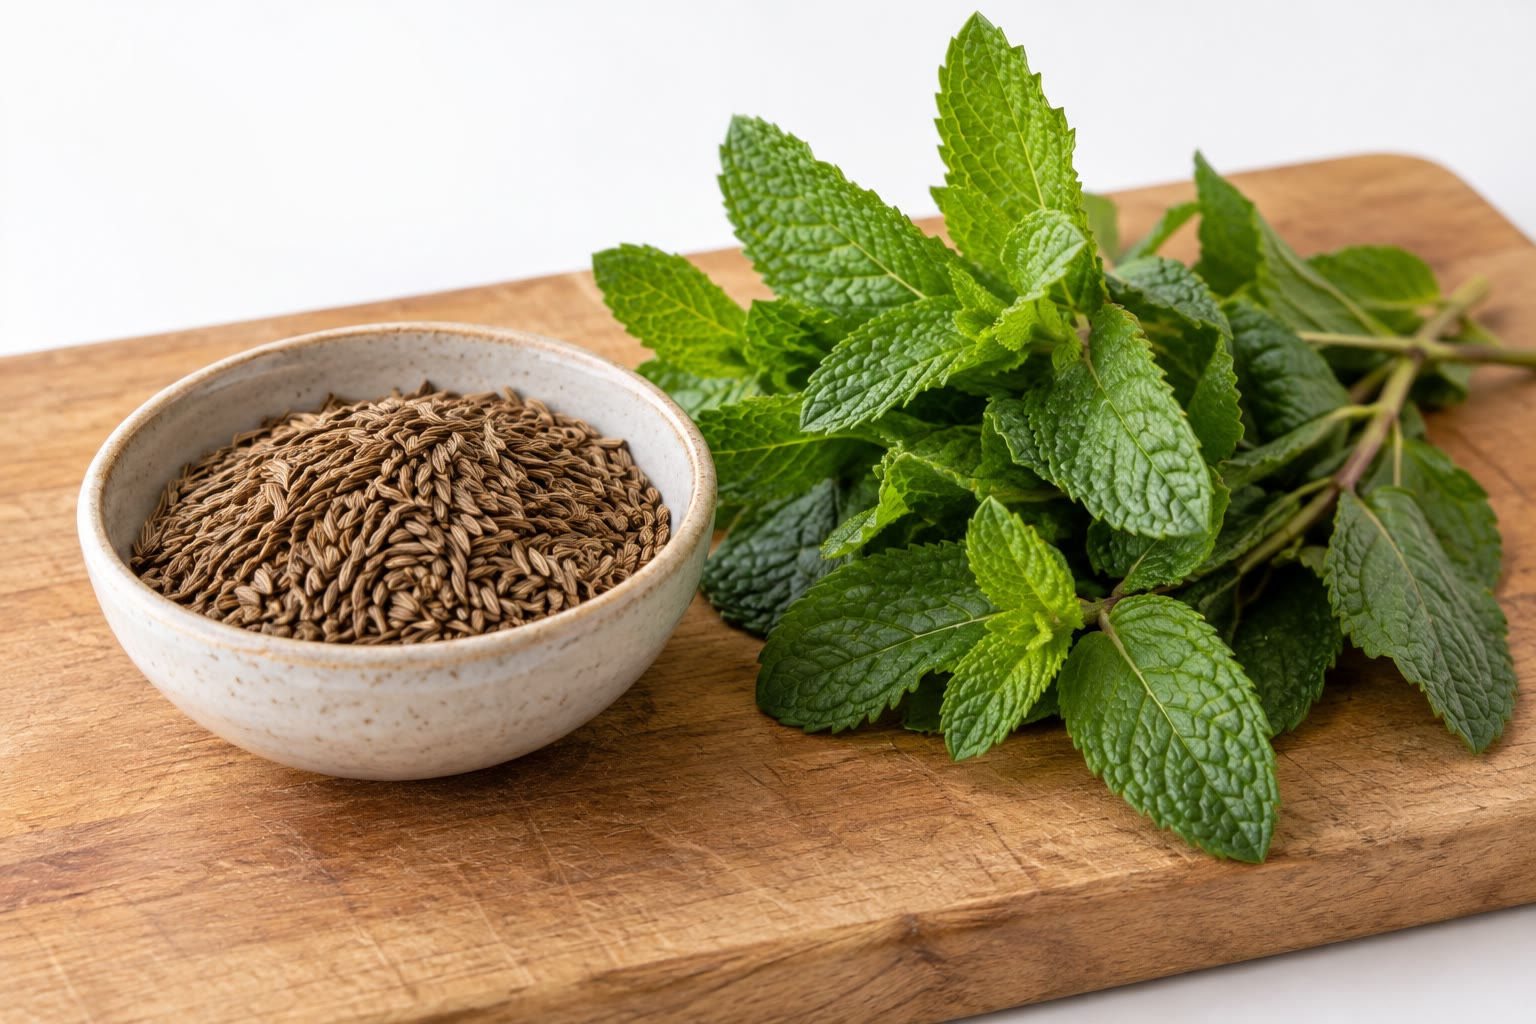
\includegraphics[width=0.55\linewidth]{images/book2/ai/b1-16-caraway-mint.jpg}

{\small Biji jintan Belanda dan daun mint hijau. Bau jintan Belanda
terutama berasal dari \cip{S}-karvon, bau mint hijau dari bayangan
cerminnya, \cip{R}-karvon.}
\end{omfigure}

\section{Isomer dan cara menggambarkannya}

\begin{definition}[Konstitusi, konfigurasi, konformasi]\label{def:b1:stereochemistry-in-depth:isomers}
Dua senyawa dengan rumus yang sama yang atom-atomnya terhubung dalam
urutan yang berbeda adalah \emph{isomer struktur}\index{isomer struktur}.
Senyawa-senyawa dengan konstitusi yang sama yang atom-atomnya hanya
berbeda dalam susunannya di ruang adalah
\emph{stereoisomer}\index{stereoisomer}. Susunan yang hanya dapat diubah
dengan memutus ikatan adalah \emph{konfigurasi}\index{konfigurasi} sebuah
stereoisomer; susunan yang diperoleh melalui rotasi mengelilingi ikatan
tunggal, tanpa memutus satu pun, adalah
\emph{konformasi}\index{konformasi}.
\end{definition}

Pada suhu kamar, rotasi mengelilingi ikatan tunggal terjadi miliaran kali
per sekon: \omterm{def:b1:stereochemistry-in-depth:isomers}{konformasi-konformasi} saling berubah dan tidak dapat
diisolasi, sedangkan \omterm{def:b1:stereochemistry-in-depth:isomers}{konfigurasi} stabil dan menghasilkan senyawa-senyawa
yang berbeda.

\begin{definition}[Cara menggambarkan]\label{def:b1:stereochemistry-in-depth:representations}
Dalam \emph{representasi Cram}\index{representasi Cram} dua ikatan
digambar pada bidang halaman, baji tebal mengarah ke pembaca dan baji
bergaris menjauhi pembaca. \emph{Proyeksi Newman}\index{proyeksi Newman}
memandang molekul sepanjang satu ikatan C--C: karbon depan berupa sebuah
titik tempat ketiga ikatan lainnya bertemu, karbon belakang berupa
lingkaran yang dari tepinya ikatan-ikatannya keluar. Dalam
\emph{proyeksi Fischer}\index{proyeksi Fischer} rantai karbon digambar
tegak, ikatan mendatar mengarah ke pembaca dan ikatan tegak menjauhi
pembaca; setiap persilangan adalah karbon stereogenik.
\end{definition}

\begin{omfigure}
\begin{tikzpicture}[font=\small]
  % staggered and eclipsed ethane, Newman
  \pic (s) at (0,0) {omnewman={90}{30}};
  \foreach \k in {1,2,3} { \node at (s-f\k) {H}; \node at (s-b\k) {H}; }
  \node at (0,-1.9) {goyang};
  \pic (e) at (3.6,0) {omnewman={90}{108}};
  \foreach \k in {1,2,3} { \node at (e-f\k) {H}; }
  \foreach \k in {1,2,3} { \node[font=\scriptsize, black!60] at ($(e-b\k)!-0.12!(e-c)$) {H}; }
  \node at (3.6,-1.9) {eklips};
  % Fischer projection of (R)-lactic acid
  \begin{scope}[xshift=7.6cm]
    \draw[thick] (-0.9,0) -- (0.9,0) (0,-0.9) -- (0,0.9);
    \node[above] at (0,0.9) {\ce{COOH}};
    \node[below] at (0,-0.9) {\ce{CH3}};
    \node[left] at (-0.9,0) {H};
    \node[right] at (0.9,0) {OH};
    \node at (0,-1.9) {Fischer};
  \end{scope}
  % Cram of the same
  \begin{scope}[xshift=11.0cm]
    \node at (0,0) {\chemfig{C(-[2]COOH)(-[:210]H_3C)(<:[:-12]OH)(<[:-55]H)}};
    \node at (0,-1.9) {Cram};
  \end{scope}
\end{tikzpicture}

{\small Kiri: \omterm{def:b1:stereochemistry-in-depth:representations}{proyeksi Newman} etana sepanjang ikatan C--C-nya, goyang
(ikatan belakang di antara ikatan-ikatan depan) dan eklips (ikatan
belakang tersembunyi di balik ikatan-ikatan depan, digambar sedikit
bergeser). Kanan: molekul yang sama, asam \cip{R}-laktat, sebagai \omterm{def:b1:stereochemistry-in-depth:representations}{proyeksi
Fischer} dan dalam \omterm{def:b1:stereochemistry-in-depth:representations}{representasi Cram} (ikatan tegak salib Fischer
menjauhi pembaca, ikatan mendatarnya mengarah ke pembaca).}
\end{omfigure}

\begin{method}[Dari Cram ke Newman]\label{met:b1:stereochemistry-in-depth:newman-from-cram}
\begin{enumerate}
  \item Pilihlah ikatan yang akan dipandang dan ujung yang lebih dekat ke
        mata.
  \item Gambarlah ketiga ikatan karbon depan dari pusat, dengan
        mempertahankan urutannya (searah atau berlawanan arah jarum jam)
        sebagaimana terlihat dari mata.
  \item Gambarlah ikatan-ikatan karbon belakang dari lingkaran, dengan
        urutannya sebagaimana terlihat dari sisi yang sama.
  \item Periksalah: memutar karbon belakang sebesar $60^\circ$ mengubah
        \omterm{def:b1:stereochemistry-in-depth:conformations}{konformasi goyang} menjadi eklips; sebesar $120^\circ$, dari satu
        \omterm{def:b1:stereochemistry-in-depth:conformations}{konformasi goyang} ke \omterm{def:b1:stereochemistry-in-depth:conformations}{konformasi goyang} berikutnya.
\end{enumerate}
\end{method}

\section{Konfigurasi: aturan CIP}

\begin{definition}[Aturan CIP, deskriptor]\label{def:b1:stereochemistry-in-depth:cip}
\emph{Aturan CIP}\index{aturan CIP} (Cahn--Ingold--Prelog) mengurutkan
keempat substituen sebuah \omterm{def:b1:stereochemistry-in-depth:stereocentre}{pusat stereogenik}: nomor atom yang lebih tinggi
lebih dahulu; jika sama, bandingkan himpunan atom yang terikat
berikutnya, dan seterusnya ke arah luar; ikatan rangkap dua dihitung
sebagai dua ikatan tunggal ke atom-atom duplikat. Dengan substituen
berperingkat terendah mengarah menjauhi mata, urutan $1 \to 2 \to 3$
yang berputar searah jarum jam mendefinisikan deskriptor \cip{R}, dan
yang berlawanan arah jarum jam \cip{S}. Untuk ikatan rangkap dua dengan
dua substituen pada setiap karbon, \cip{Z} berarti kedua substituen
berperingkat lebih tinggi berada di sisi yang sama dan \cip{E} di sisi
yang berlawanan.
\end{definition}

\begin{method}[Menentukan \texorpdfstring{\cip{R}}{(R)} atau \texorpdfstring{\cip{S}}{(S)}]\label{met:b1:stereochemistry-in-depth:cip}
\begin{enumerate}
  \item Urutkan keempat substituen menurut \omterm{def:b1:stereochemistry-in-depth:cip}{aturan CIP}.
  \item Jika substituen berperingkat terendah mengarah menjauhi pembaca
        (baji bergaris, atau ikatan tegak pada \omterm{def:b1:stereochemistry-in-depth:representations}{proyeksi Fischer}), bacalah
        putaran $1 \to 2 \to 3$ secara langsung.
  \item Jika substituen itu mengarah ke pembaca (baji tebal, ikatan
        Fischer mendatar), bacalah putarannya lalu balikkan deskriptornya.
  \item Menukar dua substituen mana pun membalikkan deskriptornya: sebuah
        pemeriksaan cepat.
\end{enumerate}
Pada asam laktat, $\ce{OH} > \ce{COOH} > \ce{CH3} > \ce{H}$ (O; lalu
C(O,O,O) mengalahkan C(H,H,H)). Pada \omterm{def:b1:stereochemistry-in-depth:representations}{proyeksi Fischer} di atas, H mendatar
(ke arah pembaca) dan $\ce{OH} \to \ce{COOH} \to \ce{CH3}$ berputar
berlawanan arah jarum jam: setelah dibalik, pusat itu \cip{R}.
\end{method}

\section{Kiralitas dan akibat-akibatnya}

\begin{definition}[Pusat stereogenik, kiralitas]\label{def:b1:stereochemistry-in-depth:stereocentre}
Sebuah benda disebut \emph{kiral}\index{kiral} jika tidak dapat
ditumpangkan tepat pada bayangan cerminnya, dan \emph{akiral}\index{akiral}
jika dapat; sifat itu disebut \emph{kiralitas}\index{kiralitas}.
\emph{Pusat stereogenik}\index{pusat stereogenik} adalah atom yang jika
dua substituennya dipertukarkan menghasilkan sebuah \omterm{def:b1:stereochemistry-in-depth:isomers}{stereoisomer}; karbon
tetrahedral dengan empat substituen yang berbeda adalah salah satunya.
\end{definition}

Molekul yang mempunyai bidang simetri atau pusat simetri bersifat \omterm{def:b1:stereochemistry-in-depth:stereocentre}{akiral};
molekul yang tidak mempunyai keduanya, dalam praktik, bersifat \omterm{def:b1:stereochemistry-in-depth:stereocentre}{kiral}.
Kriteria yang tepat, dalam bentuk operasi-operasi simetri, diberikan
dalam jilid Tahun~3.

\begin{definition}[Enantiomer, diastereomer, senyawa meso, campuran rasemat]\label{def:b1:stereochemistry-in-depth:enantiomers}
Dua \omterm{def:b1:stereochemistry-in-depth:isomers}{stereoisomer} yang saling merupakan bayangan cermin adalah
\emph{enantiomer}\index{enantiomer}; \omterm{def:b1:stereochemistry-in-depth:isomers}{stereoisomer} yang tidak demikian
adalah \emph{diastereomer}\index{diastereomer}. \emph{Senyawa
meso}\index{senyawa meso} mempunyai pusat-pusat stereogenik tetapi
\omterm{def:b1:stereochemistry-in-depth:stereocentre}{akiral}. Campuran ekuimolar dua enantiomer adalah \emph{campuran
rasemat}\index{campuran rasemat}.
\end{definition}

\begin{proposition}[Banyaknya stereoisomer]\label{prop:b1:stereochemistry-in-depth:max-stereoisomers}
Molekul dengan $n$ \omterm{def:b1:stereochemistry-in-depth:stereocentre}{pusat stereogenik} (dan tanpa unit stereogenik lain)
mempunyai paling banyak $2^n$ \omterm{def:b1:stereochemistry-in-depth:isomers}{stereoisomer}, dalam paling banyak
$2^{n-1}$ pasangan \omterm{def:b1:stereochemistry-in-depth:enantiomers}{enantiomer}; bentuk meso membuat jumlahnya lebih kecil.
\end{proposition}

\begin{proof}
Setiap pusat bersifat \cip{R} atau \cip{S} secara bebas: $2^n$ kombinasi.
Bayangan cermin mengubah setiap deskriptor, sehingga kombinasi-kombinasi
itu berpasangan menjadi \omterm{def:b1:stereochemistry-in-depth:enantiomers}{enantiomer}, $2^{n-1}$ pasangan. Jika sebuah
kombinasi sama dengan bayangan cerminnya sendiri setelah molekulnya
dirotasi (sebuah bentuk meso), pasangannya menyatu menjadi satu senyawa.
\end{proof}

Asam tartrat, \ce{HOOC-CH(OH)-CH(OH)-COOH}, mempunyai dua pusat yang
ekuivalen: \cip{R,R} dan \cip{S,S} adalah \omterm{def:b1:stereochemistry-in-depth:enantiomers}{enantiomer}, sedangkan
\cip{R,S} mempunyai bidang cermin di antara kedua karbon dan merupakan
bentuk meso: tiga \omterm{def:b1:stereochemistry-in-depth:isomers}{stereoisomer}, bukan empat.

\begin{proposition}[Sifat-sifat enantiomer]\label{prop:b1:stereochemistry-in-depth:enantiomer-properties}
Dua \omterm{def:b1:stereochemistry-in-depth:enantiomers}{enantiomer} mempunyai titik leleh dan titik didih yang sama,
\omterm{def:b1:precipitation:solubility}{kelarutan} yang sama dalam pelarut \omterm{def:b1:stereochemistry-in-depth:stereocentre}{akiral}, spektrum yang sama, dan
kereaktifan yang sama terhadap pereaksi \omterm{def:b1:stereochemistry-in-depth:stereocentre}{akiral}; keduanya berbeda dalam
pengaruhnya terhadap cahaya terpolarisasi dan dalam interaksinya dengan
molekul \omterm{def:b1:stereochemistry-in-depth:stereocentre}{kiral} lain. \omterm{def:b1:stereochemistry-in-depth:enantiomers}{Diastereomer} berbeda dalam semua sifatnya.
\end{proposition}

\begin{proof}
Setiap sifat yang hanya bergantung pada jarak dan sudut di dalam molekul,
atau antara molekul itu dan pasangan-pasangan \omterm{def:b1:stereochemistry-in-depth:stereocentre}{akiral}, sama untuk sebuah
benda dan bayangan cerminnya, karena pencerminan mempertahankan jarak
dan sudut. Pasangan yang \omterm{def:b1:stereochemistry-in-depth:stereocentre}{kiral} (sebuah reseptor, pereaksi \omterm{def:b1:stereochemistry-in-depth:stereocentre}{kiral}, jalan
heliks cahaya terpolarisasi yang dipaparkan di bawah) membentuk pasangan
yang bersifat \omterm{def:b1:stereochemistry-in-depth:enantiomers}{diastereomer}, bukan lagi bayangan cermin, yang karena itu
berbeda. \omterm{def:b1:stereochemistry-in-depth:enantiomers}{Diastereomer} tidak dihubungkan oleh pencerminan apa pun: jarak
internalnya berbeda.
\end{proof}

\begin{omfigure}
\begin{tikzpicture}[font=\small, line join=round]
  \foreach \dx/\kind/\lab in {0/1/{\cip{R}-karvon (mint hijau)}, 5.2/0/{\cip{S}-karvon (jintan Belanda)}} {
  \begin{scope}[xshift=\dx cm]
    \coordinate (c1) at (0,1); \coordinate (c2) at (0.87,0.5);
    \coordinate (c3) at (0.87,-0.5); \coordinate (c4) at (0,-1);
    \coordinate (c5) at (-0.87,-0.5); \coordinate (c6) at (-0.87,0.5);
    \draw[thick] (c1) -- (c2) -- (c3) -- (c4) -- (c5) -- (c6) -- cycle;
    \draw[thick] ($(c2)!0.15!(c3)+(-0.12,0)$) -- ($(c3)!0.15!(c2)+(-0.12,0)$);
    \draw[thick] (c1) -- ++(0,0.7) node[above] {O};
    \draw[thick] ($(c1)+(0.1,0)$) -- ++(0,0.62);
    \draw[thick] (c2) -- ++(0.75,0.43) node[right] {\ce{CH3}};
    \coordinate (q) at ($(c5)+(-0.75,-0.43)$);
    \ifnum\kind=1
      \fill (c5) -- ($(q)+(0.06,-0.1)$) -- ($(q)+(-0.06,0.1)$) -- cycle;
    \else
      \foreach \t in {0.15,0.3,0.45,0.6,0.75,0.9}
        \draw ($(c5)!\t!(q)+(\t*0.06,-\t*0.1)$) -- ($(c5)!\t!(q)+(-\t*0.06,\t*0.1)$);
    \fi
    \draw[thick] (q) -- ++(-0.6,0.5) node[above] {\ce{CH2}};
    \draw[thick] ($(q)+(0.08,0.06)$) -- ++(-0.6,0.5);
    \draw[thick] (q) -- ++(0,-0.75) node[below] {\ce{CH3}};
    \node[font=\scriptsize] at ($(c5)+(0.35,0.12)$) {5};
    \node at (0,-2.85) {\lab};
  \end{scope}}
\end{tikzpicture}

{\small Kedua karvon, digambar pada kerangka yang sama: gugus isopropenil
pada C5 mengarah ke pembaca (baji tebal) pada yang satu dan menjauhi
pembaca (baji bergaris) pada yang lain, dengan hidrogen C5 (tidak
digambar) di sisi yang berlawanan. Keduanya saling merupakan bayangan
cermin: \omterm{def:b1:stereochemistry-in-depth:enantiomers}{enantiomer} (\cref{exo:b1:stereochemistry-in-depth:4}).}
\end{omfigure}

\begin{history}[Karbon tetrahedral]
\begin{minipage}[t]{0.2\linewidth}\vspace{0pt}
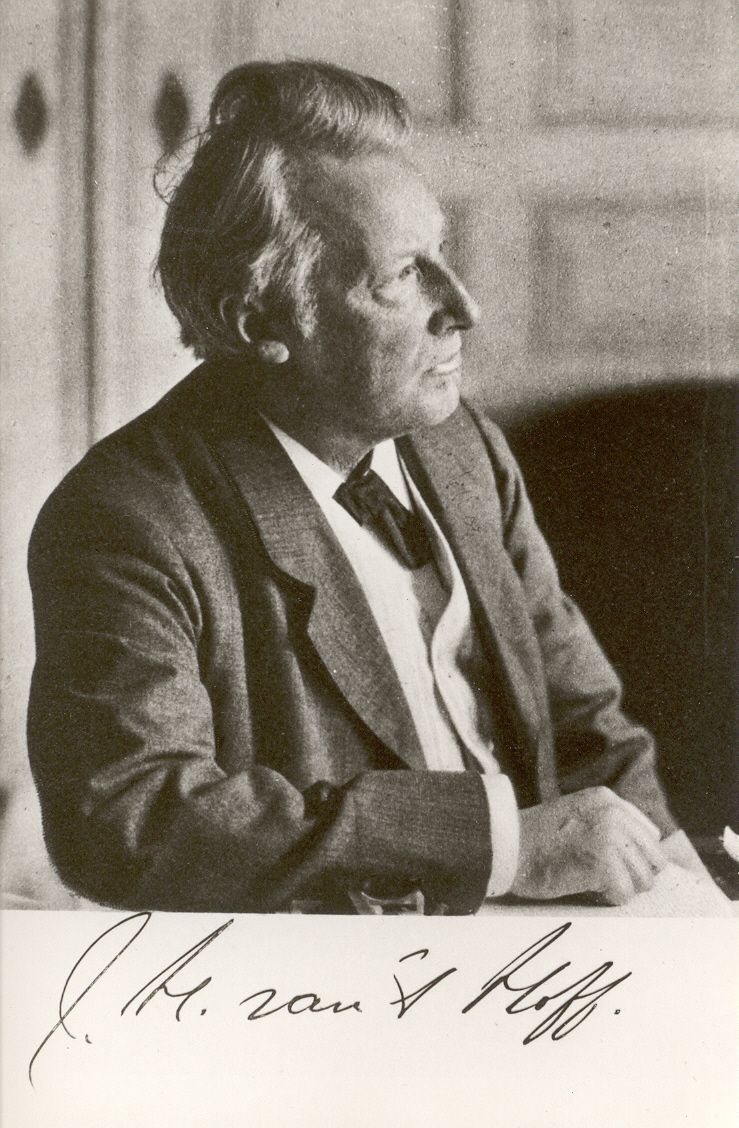
\includegraphics[width=\linewidth]{images/book2/van-t-hoff.jpg}
\end{minipage}\hfill
\begin{minipage}[t]{0.76\linewidth}\vspace{0pt}
Jacobus Henricus van 't Hoff mengusulkan, ketika masih menjadi ahli kimia
muda, bahwa keempat ikatan sebuah atom karbon mengarah ke sudut-sudut
sebuah tetrahedron. Karbon dengan empat substituen yang berbeda lalu
terdapat dalam dua susunan yang saling merupakan bayangan cermin, yang
menjelaskan mengapa sebagian senyawa terdapat dalam dua bentuk yang hanya
berbeda dalam cara memutar cahaya terpolarisasi. Gagasan itu adalah titik
awal setiap gambar dalam bab ini. (Foto diterbitkan pada tahun 1911,
domain publik, Wikimedia Commons.)
\end{minipage}
\end{history}

\section{Konformasi}

\begin{definition}[Sudut torsi dan konformasi]\label{def:b1:stereochemistry-in-depth:conformations}
Untuk empat atom A--B--C--D, \emph{sudut torsi}\index{sudut torsi}
$\theta$ mengelilingi B--C adalah sudut antara bidang ABC dan BCD, yang
dibaca pada \omterm{def:b1:stereochemistry-in-depth:representations}{proyeksi Newman} sepanjang B--C. Sebuah \omterm{def:b1:stereochemistry-in-depth:isomers}{konformasi} adalah
\emph{konformasi eklips}\index{konformasi eklips} jika ikatan-ikatan
karbon depan dan belakang segaris dalam proyeksi, dan \emph{konformasi
goyang}\index{konformasi goyang} jika berselang-seling. Pada butana,
dipandang sepanjang C2--C3, \omterm{def:b1:stereochemistry-in-depth:isomers}{konformasi} goyang dengan kedua gugus metil
pada $180^\circ$ adalah \emph{konformasi anti}\index{konformasi anti},
sedangkan yang pada $\pm 60^\circ$ adalah \emph{konformasi
gauche}\index{konformasi gauche}. Pada sikloheksana, cincin terlipat yang
bebas tegangan adalah \emph{kursi}\index{kursi}; setiap karbon membawa
satu ikatan \emph{aksial}\index{aksial}, sejajar dengan sumbu cincin, dan
satu ikatan \emph{ekuatorial}\index{ekuatorial}, kira-kira pada bidang
tengah cincin. \emph{Pembalikan cincin}\index{pembalikan cincin} mengubah
satu kursi menjadi kursi yang lain, setiap ikatan aksial menjadi
ekuatorial dan sebaliknya.
\end{definition}

\begin{omfigure}
\begin{tikzpicture}
\begin{axis}[
  width=0.82\linewidth, height=5.8cm, xmin=0, xmax=360, ymin=0, ymax=21,
  legend style={font=\scriptsize, draw=none, at={(0.5,0.62)}, anchor=center},
  axis x line=bottom, axis y line=left, xlabel={sudut torsi $\theta$ (derajat)},
  ylabel={energi (kJ/mol)}, xtick={0,60,120,180,240,300,360},
  tick label style={font=\small}, label style={font=\small}]
\addplot[omDef, very thick] table[x=theta, y=butane] {figdata/out/bachelor-1-butane-torsion.dat};
\addplot[omProp, thick, dashed] table[x=theta, y=ethane] {figdata/out/bachelor-1-butane-torsion.dat};
\node[font=\scriptsize, anchor=south west] at (axis cs:0,18.4) {sin};
\node[font=\scriptsize, anchor=south] at (axis cs:62,18.4) {gauche};
\node[font=\scriptsize, anchor=south] at (axis cs:120,18.4) {eklips};
\node[font=\scriptsize, anchor=south] at (axis cs:180,18.4) {anti};
\node[font=\scriptsize, anchor=south] at (axis cs:240,18.4) {eklips};
\node[font=\scriptsize, anchor=south] at (axis cs:298,18.4) {gauche};
\node[font=\scriptsize, anchor=south east] at (axis cs:360,18.4) {sin};
\legend{butana, etana}
\end{axis}
\end{tikzpicture}

{\small Energi torsi butana mengelilingi ikatan tengahnya (garis utuh;
$\theta
= 0$ ketika kedua gugus metil saling menutupi) dan etana (putus-putus),
yang dihitung dari potensial torsi eksperimen. Etana: sawar
\qty{12.2}{kJ/mol}. Butana: anti paling stabil; gauche \qty{2.8}{kJ/mol}
lebih tinggi, pada $\theta = 62^\circ$; sawar \qty{15.2}{kJ/mol} (metil
menutupi hidrogen) dan \qty{16.5}{kJ/mol} (metil menutupi metil).}
% ledger: rot:ethane-V3, rot:butane-V1, rot:butane-V2, rot:butane-V3, rot:butane-V4, rot:butane-V5, rot:butane-V6 (curves in figdata/bachelor-1/butane-torsion.py)
\end{omfigure}

Sawar-sawar itu kecil dibandingkan dengan energi termal yang tersedia
dalam tumbukan ($RT = \qty{2.5}{kJ/mol}$ pada suhu kamar, dan jauh lebih
besar di ekor distribusinya, \cref{ch:b1:elementary-steps}): rotasi
berlangsung cepat, dan butana adalah campuran molekul anti dan gauche
yang tidak dapat dipisahkan.

\begin{method}[Menggambar kursi]\label{met:b1:stereochemistry-in-depth:draw-chair}
\begin{enumerate}
  \item Gambarlah dua garis sejajar yang sedikit miring ke bawah ke kanan,
        dengan posisi bergeser; hubungkan ujung-ujungnya dengan huruf V di
        kiri dan huruf V terbalik di kanan untuk menutup cincin beranggota
        enam.
  \item Ikatan \omterm{def:b1:stereochemistry-in-depth:conformations}{aksial} tegak: ke atas pada karbon yang mengarah ke atas, ke
        bawah pada karbon yang mengarah ke bawah, berselang-seling di
        sekeliling cincin.
  \item Ikatan \omterm{def:b1:stereochemistry-in-depth:conformations}{ekuatorial} sejajar dengan ikatan cincin yang berjarak satu
        ikatan, dan mengarah ke luar.
  \item Untuk membalik cincin, gambarlah \omterm{def:b1:stereochemistry-in-depth:conformations}{kursi} yang lain; substituen yang
        \omterm{def:b1:stereochemistry-in-depth:conformations}{aksial} pada \omterm{def:b1:stereochemistry-in-depth:conformations}{kursi} yang satu menjadi \omterm{def:b1:stereochemistry-in-depth:conformations}{ekuatorial} pada \omterm{def:b1:stereochemistry-in-depth:conformations}{kursi} yang
        lain.
\end{enumerate}
\end{method}

\begin{omfigure}
\begin{tikzpicture}[font=\small]
  \pic (a) at (0,0) {omchair};
  \foreach \k in {1,2,3,4,5,6} \draw[omProp, thick] (a-c\k) -- (a-a\k);
  \foreach \k in {1,2,3,4,5,6} \draw[omDef, thick] (a-c\k) -- (a-e\k);
  \node[omProp, anchor=south] at (a-a3) {aksial};
  \node[omDef, anchor=north] at (a-e5) {ekuatorial};
  \begin{scope}[xshift=4.9cm]
    \pic (b) at (0,0) {omchair};
    \draw[thick] (b-c1) -- (b-e1) node[right] {\ce{CH3}};
    \draw[thick] (b-c1) -- (b-a1) node[above] {H};
    \node at (0,-1.5) {\ce{CH3} ekuatorial};
  \end{scope}
  \draw[<->, thick] (8.1,0) -- (8.8,0) node[midway, above] {balik};
  \begin{scope}[xshift=10.45cm]
    \pic (c) at (0,0) {omchairflip};
    \draw[thick] (c-c4) -- (c-a4) node[below] {\ce{CH3}};
    \draw[thick] (c-c4) -- (c-e4) node[right] {H};
    \node at (0,-1.5) {\ce{CH3} aksial};
  \end{scope}
\end{tikzpicture}

{\small Kiri: \omterm{def:b1:stereochemistry-in-depth:conformations}{kursi} sikloheksana dengan keenam ikatan \omterm{def:b1:stereochemistry-in-depth:conformations}{aksialnya} (jingga,
berselang-seling ke atas dan ke bawah) dan keenam ikatan \omterm{def:b1:stereochemistry-in-depth:conformations}{ekuatorialnya}
(biru). Kanan: kedua \omterm{def:b1:stereochemistry-in-depth:conformations}{kursi} metilsikloheksana, yang saling berubah melalui
\omterm{def:b1:stereochemistry-in-depth:conformations}{pembalikan cincin}; gugus metilnya \omterm{def:b1:stereochemistry-in-depth:conformations}{ekuatorial} pada yang satu, \omterm{def:b1:stereochemistry-in-depth:conformations}{aksial} pada
yang lain.}
\end{omfigure}

\begin{proposition}[Substituen ekuatorial lebih disukai]\label{prop:b1:stereochemistry-in-depth:chair-substituent}
Pada sikloheksana monosubstitusi, \omterm{def:b1:stereochemistry-in-depth:conformations}{kursi} dengan substituen \omterm{def:b1:stereochemistry-in-depth:conformations}{ekuatorial}
lebih stabil. Untuk gugus metil, posisi aksial menambahkan dua interaksi
gauche dengan karbon-karbon cincin, masing-masing senilai interaksi pada
butana (\qtyrange{2.8}{2.9}{kJ/mol}), sekitar \qty{5.7}{kJ/mol}
seluruhnya: sebuah perkiraan selisih energinya.
\end{proposition}

\begin{proof}
Dipandang sepanjang ikatan C1--C2, metil \omterm{def:b1:stereochemistry-in-depth:conformations}{aksial} pada C1 bersifat gauche
terhadap C3 cincin; dipandang sepanjang C1--C6, gauche terhadap C5: dua
interaksi gauche yang mirip butana, yang juga terlihat sebagai
berdesakannya metil dengan hidrogen-hidrogen \omterm{def:b1:stereochemistry-in-depth:conformations}{aksial} pada C3 dan C5
(interaksi 1,3-diaksial). Metil \omterm{def:b1:stereochemistry-in-depth:conformations}{ekuatorial} bersifat anti terhadap C3 dan
C5. Setiap interaksi gauche bernilai sama seperti pada butana,
\qty{2.8}{kJ/mol} dalam potensial torsi pada gambar.
\end{proof}

Dengan $\Delta E = \qty{5.7}{kJ/mol}$, rasio \omterm{def:b1:stereochemistry-in-depth:conformations}{kursi} \omterm{def:b1:stereochemistry-in-depth:conformations}{ekuatorial} terhadap
\omterm{def:b1:stereochemistry-in-depth:conformations}{kursi} \omterm{def:b1:stereochemistry-in-depth:conformations}{aksial} pada \qty{25}{\celsius} adalah $\exp(\Delta E/RT) = 10$:
sekitar \qty{91}{\percent} \omterm{def:b1:stereochemistry-in-depth:conformations}{ekuatorial}
(\cref{exo:b1:stereochemistry-in-depth:9}). Gugus-gugus besar, seperti
tert-butil, mengunci cincin pada \omterm{def:b1:stereochemistry-in-depth:conformations}{kursi} tempat gugus itu \omterm{def:b1:stereochemistry-in-depth:conformations}{ekuatorial}.

\section{Aktivitas optis}

\begin{definition}[Aktivitas optis, rotasi spesifik]\label{def:b1:stereochemistry-in-depth:optical-activity}
Sebuah zat menunjukkan \emph{aktivitas optis}\index{aktivitas optis} jika
memutar bidang polarisasi cahaya terpolarisasi linear yang melewatinya.
Dilihat oleh pengamat yang menghadap cahaya, zat
\emph{dekstrorotatori}\index{dekstrorotatori}, yang ditulis $(+)$,
memutarnya searah jarum jam, dan zat
\emph{levorotatori}\index{levorotatori}, $(-)$, berlawanan arah jarum
jam. \emph{Rotasi spesifik}\index{rotasi spesifik} adalah
$[\alpha] = \alpha/(\ell c)$, dengan $\alpha$ sudut terukur dalam
derajat, $\ell$ panjang lintasan dalam desimeter, dan $c$ konsentrasi
massa dalam \unit{g/mL}; rotasi spesifik bergantung pada panjang
gelombang (biasanya garis kuning natrium), suhu, dan pelarut.
\end{definition}

\begin{omfigure}
\begin{tikzpicture}[font=\small, >={Stealth}]
  \fill[yellow!70!orange] (0,0) circle (0.25);
  \node[below] at (0,-0.45) {lampu};
  \draw[thick] (1.3,-0.7) rectangle (1.45,0.7); \node[below] at (1.37,-0.75) {polarisator};
  \draw[omDef!20, fill=omDef!10] (2.4,-0.45) rectangle (5.6,0.45);
  \node at (4.0,0) {sampel, panjang $\ell$};
  \draw[thick] (6.5,-0.7) rectangle (6.65,0.7); \node[below] at (6.57,-0.75) {analisator};
  \draw (7.6,0) circle (0.3); \node[below] at (7.6,-0.45) {mata};
  \draw[->, orange!80!black] (0.3,0) -- (1.25,0);
  \draw[->, orange!80!black] (1.5,0) -- (2.35,0);
  \draw[->, orange!80!black] (5.65,0) -- (6.45,0);
  % polarisation planes
  \draw[thick, omThm] (1.9,-0.35) -- (1.9,0.35);
  \draw[thick, omThm] (6.05,-0.33) -- ++(70:0.0) -- (5.93,0.33);
  \draw[->, omThm] (5.75,0.55) arc[start angle=100, end angle=70, radius=0.6];
  \node[omThm, above] at (6.1,0.75) {$\alpha$};
\end{tikzpicture}

{\small Sebuah polarimeter. Polarisator meneruskan cahaya yang bergetar
pada satu bidang; sampel \omterm{def:b1:stereochemistry-in-depth:stereocentre}{kiral} memutar bidang itu sebesar $\alpha$;
analisator diputar sampai cahaya padam kembali, yang mengukur $\alpha$.}
\end{omfigure}

\begin{proposition}[Hukum Biot]\label{prop:b1:stereochemistry-in-depth:biot}
Untuk larutan encer beberapa zat terlarut yang aktif optis, sudut
putarnya bersifat aditif, $\alpha = \ell\sum_i [\alpha]_i c_i$
(\emph{hukum Biot}\index{hukum Biot}). Dua \omterm{def:b1:stereochemistry-in-depth:enantiomers}{enantiomer} mempunyai \omterm{def:b1:stereochemistry-in-depth:optical-activity}{rotasi
spesifik} yang berlawanan; \omterm{def:b1:stereochemistry-in-depth:enantiomers}{campuran rasemat} tidak memutar cahaya.
\end{proposition}

\begin{proof}
Dalam larutan encer setiap zat terlarut menyumbang secara bebas,
sebanding dengan banyaknya molekul yang dilewati, yaitu dengan
$\ell c_i$; inilah isi eksperimental hukum itu. Pencerminan mengubah
searah jarum jam menjadi berlawanan arah jarum jam: molekul bayangan
cermin memutar bidang itu dengan sudut yang berlawanan, dan dalam
\omterm{def:b1:stereochemistry-in-depth:enantiomers}{campuran rasemat} kedua sumbangan itu saling meniadakan.
\end{proof}

Untuk campuran dua \omterm{def:b1:stereochemistry-in-depth:enantiomers}{enantiomer} dengan konsentrasi total $c$, bagian $x$
bentuk $(-)$ memberikan $\alpha = \ell c[\alpha]_{(-)}(x - (1 - x)) =
\ell c[\alpha]_{(-)}(2x - 1)$: mengukur $\alpha$ memberikan komposisinya.
Rotasi optis tidak terkait secara sederhana dengan deskriptornya:
senyawa \cip{R} dapat bersifat $(+)$ atau $(-)$; \cip{R}-karvon pada
mint hijau bersifat \omterm{def:b1:stereochemistry-in-depth:optical-activity}{levorotatori}.

\section{Latihan}

\begin{exercise}[$\star$]\label{exo:b1:stereochemistry-in-depth:1}
Golongkan setiap pasangan berikut sebagai \omterm{def:b1:stereochemistry-in-depth:isomers}{isomer struktur}, \omterm{def:b1:stereochemistry-in-depth:enantiomers}{enantiomer},
\omterm{def:b1:stereochemistry-in-depth:enantiomers}{diastereomer}, atau dua \omterm{def:b1:stereochemistry-in-depth:isomers}{konformasi} dari satu senyawa: butan-1-ol dan
butan-2-ol; \cip{R}- dan \cip{S}-butan-2-ol; \cip{Z}- dan
\cip{E}-but-2-ena; \omterm{def:b1:stereochemistry-in-depth:conformations}{konformasi anti} dan gauche butana; asam \cip{R,R}- dan
\cip{R,S}-tartrat.
\end{exercise}

\begin{exercise}[$\star$]\label{exo:b1:stereochemistry-in-depth:2}
Urutkan menurut \omterm{def:b1:stereochemistry-in-depth:cip}{aturan CIP}: \ce{-OH}, \ce{-NH2}, \ce{-CH3}, \ce{-H};
lalu \ce{-CH2OH}, \ce{-CHO}, \ce{-COOH}, \ce{-CH(CH3)2}; lalu \ce{-Cl},
\ce{-CH2Cl}, \ce{-CCl3}, \ce{-Br}.
\end{exercise}

\begin{exercise}[$\star$]\label{exo:b1:stereochemistry-in-depth:3}
Berapa banyak \omterm{def:b1:stereochemistry-in-depth:isomers}{stereoisomer} yang dimiliki 2,3-diklorobutana,
2-bromo-3-klorobutana, dan pentana-2,4-diol? Tentukan bentuk-bentuk
mesonya.
\end{exercise}

\begin{exercise}[$\star$]\label{exo:b1:stereochemistry-in-depth:4}
Urutkan keempat substituen C5 karvon menurut \omterm{def:b1:stereochemistry-in-depth:cip}{aturan CIP} dan periksalah
deskriptor yang diberikan pada gambar kedua karvon (baji tebal: gugus
isopropenil ke arah pembaca, H menjauhi pembaca).
\end{exercise}

\begin{exercise}[$\star\star$]\label{exo:b1:stereochemistry-in-depth:5}
Gambarlah \omterm{def:b1:stereochemistry-in-depth:representations}{proyeksi Newman} butana sepanjang C2--C3 pada $\theta = 0$, 60,
120, dan $180^\circ$, lalu bacalah energinya pada kurva. Berapa bagian
molekul yang akan bersifat gauche seandainya energi gauche dan anti sama?
\end{exercise}

\begin{exercise}[$\star\star$]\label{exo:b1:stereochemistry-in-depth:6}
Gambarlah \omterm{def:b1:stereochemistry-in-depth:representations}{proyeksi Fischer} \cip{S}-alanina,
\ce{H2N-CH(CH3)-COOH}, dengan gugus asam di atas. Di sisi manakah gugus
aminonya?
\end{exercise}

\begin{exercise}[$\star\star$]\label{exo:b1:stereochemistry-in-depth:7}
Tunjukkan bahwa \textit{cis}-1,2-dimetilsikloheksana mempunyai satu metil
\omterm{def:b1:stereochemistry-in-depth:conformations}{aksial} dan satu \omterm{def:b1:stereochemistry-in-depth:conformations}{ekuatorial} pada kedua \omterm{def:b1:stereochemistry-in-depth:conformations}{kursinya}, sedangkan isomer
\textit{trans} mempunyai satu \omterm{def:b1:stereochemistry-in-depth:conformations}{kursi} dengan keduanya \omterm{def:b1:stereochemistry-in-depth:conformations}{ekuatorial}. Isomer
manakah yang lebih stabil? Gunakan perkiraan dalam bab ini.
\end{exercise}

\begin{exercise}[$\star\star$]\label{exo:b1:stereochemistry-in-depth:8}
Larutan sebuah senyawa \omterm{def:b1:stereochemistry-in-depth:stereocentre}{kiral} \qty{0.100}{g/mL} dalam tabung
\qty{2.00}{dm} memutar cahaya sebesar $+13.2^\circ$. Hitunglah $[\alpha]$.
Berapa yang akan diberikan tabung \qty{1.00}{dm}? Dan \omterm{def:b1:stereochemistry-in-depth:enantiomers}{enantiomernya} pada
konsentrasi yang sama?
\end{exercise}

\begin{exercise}[$\star\star$]\label{exo:b1:stereochemistry-in-depth:9}
Dengan $\Delta E = \qty{5.7}{kJ/mol}$ dan rasio Boltzmann
$\exp(\Delta E/RT)$, hitunglah bagian \omterm{def:b1:stereochemistry-in-depth:conformations}{kursi} metilsikloheksana dengan
metil \omterm{def:b1:stereochemistry-in-depth:conformations}{ekuatorial} pada \qty{25}{\celsius} dan pada \qty{-50}{\celsius}.
\end{exercise}

\begin{exercise}[$\star\star\star$]\label{exo:b1:stereochemistry-in-depth:10}
Jelaskan mengapa etana hanya mempunyai satu jenis \omterm{def:b1:stereochemistry-in-depth:conformations}{konformasi goyang}
sedangkan butana dua (anti dan gauche), dan mengapa gauche kurang stabil.
Dengan energi-energi pada gambar, perkirakan rasio populasi anti : gauche
butana pada \qty{25}{\celsius} (dua \omterm{def:b1:stereochemistry-in-depth:conformations}{konformasi gauche}, satu anti).
\end{exercise}

\begin{exercise}[$\star\star\star$]\label{exo:b1:stereochemistry-in-depth:11}
Tinjaulah asam 2,3,4-trihidroksipentanadioat,
\ce{HOOC-CH(OH)-CH(OH)-CH(OH)-COOH}. Hitunglah pusat-pusat
stereogeniknya, tunjukkan bahwa karbon tengah hanya stereogenik jika
kedua karbon luar mempunyai deskriptor yang berlawanan
(pseudoasimetris), lalu hitunglah \omterm{def:b1:stereochemistry-in-depth:isomers}{stereoisomernya} (termasuk bentuk
meso).
\end{exercise}

\begin{exercise}[$\star\star\star$]\label{exo:b1:stereochemistry-in-depth:12}
Sebuah sampel satu \omterm{def:b1:stereochemistry-in-depth:enantiomers}{enantiomer} sebuah senyawa ($[\alpha] = +66.0^\circ$
untuk senyawa murni pada kondisi yang dipakai) telah sebagian
terasemisasi: pada \qty{0.050}{g/mL} dalam tabung \qty{1.00}{dm} sampel
itu memberikan $+2.31^\circ$. Hitunglah bagian kedua \omterm{def:b1:stereochemistry-in-depth:enantiomers}{enantiomernya}.
\end{exercise}

\section{Soal: Mentol, Molekul yang Menyejukkan}

\begin{problem}[{Soal akhir pekan --- ketiga pusat stereo mentol,
kedelapan stereoisomernya, kursi yang serba ekuatorial, hukum Biot, dan
persentase (\textminus)-mentol dalam sampel yang sebagian terasemisasi}]
\label{pb:b1:stereochemistry-in-depth:1}
Mentol, 2-isopropil-5-metilsikloheksan-1-ol, memberikan rasa sejuk pada
mint. Senyawa alaminya adalah $(-)$-mentol, dengan \omterm{def:b1:stereochemistry-in-depth:isomers}{konfigurasi}
\cip{1R,2S,5R}. Sebuah laboratorium mengukur dengan polarimeter (garis
natrium, \qty{25}{\celsius}, etanol, $\ell = \qty{1.00}{dm}$): sampel
acuannya, $(-)$-mentol murni pada $c = \qty{0.0500}{g/mL}$, memberikan
$\alpha =
-2.46^\circ$; sampel yang diuji, pada konsentrasi yang sama, memberikan
$-1.97^\circ$.

\medskip
\noindent\textbf{Bagian I --- Pusat-pusat stereo.}
\begin{enumerate}
  \item Gambarlah konstitusi mentol dan tandai karbon-karbon
        stereogeniknya.
  \item Berapa banyak \omterm{def:b1:stereochemistry-in-depth:isomers}{stereoisomer} yang mungkin? Berapa pasangan
        \omterm{def:b1:stereochemistry-in-depth:enantiomers}{enantiomer}?
  \item Mengapa tidak ada bentuk meso?
  \item Urutkan substituen-substituen C1 menurut \omterm{def:b1:stereochemistry-in-depth:cip}{aturan CIP}.
  \item Urutkan substituen-substituen C2.
  \item Urutkan substituen-substituen C5.
  \item Tuliskan \omterm{def:b1:stereochemistry-in-depth:isomers}{konfigurasi} \omterm{def:b1:stereochemistry-in-depth:enantiomers}{enantiomer} $(-)$-mentol.
\end{enumerate}

\medskip
\noindent\textbf{Bagian II --- \omterm{def:b1:stereochemistry-in-depth:conformations}{Kursi}.}
\begin{enumerate}[resume]
  \item Gambarlah sebuah \omterm{def:b1:stereochemistry-in-depth:conformations}{kursi} sikloheksana dan tempatkan ketiga substituen
        $(-)$-mentol semuanya \omterm{def:b1:stereochemistry-in-depth:conformations}{ekuatorial}. Periksalah bahwa hal ini
        bersesuaian dengan susunan relatif (1,2-\textit{trans} dan
        1,5-\textit{cis}) mentol.
  \item Apa yang terjadi pada ketiga substituen itu pada \omterm{def:b1:stereochemistry-in-depth:conformations}{kursi} yang
        dibalik?
  \item Dengan perkiraan dalam bab ini untuk satu metil \omterm{def:b1:stereochemistry-in-depth:conformations}{aksial}, jelaskan
        mengapa mentol hampir seluruhnya berada dalam satu \omterm{def:b1:stereochemistry-in-depth:conformations}{kursi}.
  \item Neomentol hanya berbeda dari mentol pada C1. Apakah neomentol
        \omterm{def:b1:stereochemistry-in-depth:enantiomers}{enantiomer} atau \omterm{def:b1:stereochemistry-in-depth:enantiomers}{diastereomer} mentol?
  \item Pada \omterm{def:b1:stereochemistry-in-depth:conformations}{kursi} terbaik neomentol, gugus manakah yang \omterm{def:b1:stereochemistry-in-depth:conformations}{aksial}?
  \item Mengapa mentol dan neomentol mempunyai titik didih yang berbeda,
        sedangkan kedua \omterm{def:b1:stereochemistry-in-depth:enantiomers}{enantiomer} mentol tidak?
\end{enumerate}

\medskip
\noindent\textbf{Bagian III --- Rotasi optis.}
\begin{enumerate}[resume]
  \item Hitunglah $[\alpha]$ sampel acuan itu. Bandingkan dengan rentang
        $-45^\circ$ sampai $-51^\circ$ yang diberikan sebuah buku pegangan
        untuk $(-)$-mentol.
  \item Berapa $[\alpha]$ $(+)$-mentol? Mentol rasemat?
  \item Hitunglah $[\alpha]$ sampel yang diuji.
  \item Tuliskan \omterm{prop:b1:stereochemistry-in-depth:biot}{hukum Biot} untuk campuran kedua \omterm{def:b1:stereochemistry-in-depth:enantiomers}{enantiomer}, dengan $x$
        bagian $(-)$-mentol.
  \item Nyatakan $x$ sebagai fungsi rotasi terukur dan rotasi acuan.
  \item Dapatkah pengotor \omterm{def:b1:stereochemistry-in-depth:stereocentre}{kiral} dari senyawa lain mendistorsi
        pengukurannya? Berikan sebuah pemeriksaan.
\end{enumerate}

\medskip
\noindent\textbf{Bagian IV --- Komposisinya.}
\begin{enumerate}[resume]
  \item Hitunglah bagian $(-)$-mentol dalam sampel yang diuji.
  \item Sampel dari pemasok kedua memberikan $-2.40^\circ$ pada kondisi
        yang sama. Hitunglah komposisinya.
  \item Sampel manakah yang lebih dekat dengan mentol alami?
  \item Dengan tabung \qty{2.00}{dm}, sudut berapakah yang akan diberikan
        sampel yang diuji, dan mengapa tabung yang lebih panjang lebih
        baik?
  \item Nyatakan persentase $(-)$-mentol dalam sampel yang diuji, sampai
        tiga angka penting.
\end{enumerate}
\end{problem}
